\documentclass[12pt, twoside]{article}
\documentclass[12pt, twoside]{article}
\usepackage[letterpaper, margin=1in, headsep=0.2in]{geometry}
\setlength{\headheight}{0.6in}
%\usepackage[english]{babel}
\usepackage[utf8]{inputenc}
\usepackage{microtype}
\usepackage{amsmath}
\usepackage{amssymb}
%\usepackage{amsfonts}
\usepackage{siunitx} %units in math. eg 20\milli\meter
\usepackage{yhmath} % for arcs, overparenth command
\usepackage{tikz} %graphics
\usetikzlibrary{quotes, angles}
\usepackage{graphicx} %consider setting \graphicspath{{images/}}
\usepackage{parskip} %no paragraph indent
\usepackage{enumitem}
\usepackage{multicol}
\usepackage{venndiagram}

\usepackage{fancyhdr}
\pagestyle{fancy}
\fancyhf{}
\renewcommand{\headrulewidth}{0pt} % disable the underline of the header
\raggedbottom
\hfuzz=2mm %suppresses overfull box warnings

\usepackage{hyperref}
\usepackage{float}

\title{Algebra 2}
\author{Chris Huson}
\date{November 2024}

\fancyhead[LE]{\thepage}
\fancyhead[RO]{\thepage \\ First and last name: \hspace{2.5cm} \,\\ Section: \hspace{2.5cm} \,}
\fancyhead[LO]{BECA / Huson / Algebra 2: Polynomials \\* 6 November 2024}

\begin{document}

\subsubsection*{PreTest: Polynomial and rational expressions \hfill A2.A.APR.6}
\begin{enumerate}[itemsep=0.5cm]

\item Given $x \ne -3$, which expression is equivalent to $\displaystyle \frac{2x^3 + 3x^2 - 4x + 5}{x+3}$? %August 2023 Regents
    \begin{enumerate}
        \item $\displaystyle 2x^3 + 9x^2 + 23x + 74$
        \item $\displaystyle 2x^2 - 3x + 5 - \frac{10}{x+3}$
        \item $\displaystyle 2x^3 -3x^2 + 5x - 10$
        \item $\displaystyle 2x^3 + 9x + 23 + \frac{74}{x+3}$
    \end{enumerate}\vspace{3cm}

\item What is the solution set of the equation \(\displaystyle \frac{4}{k^2-8k+12} = \frac{k}{k-2} + \frac{1}{k-6} \)? %August 2022 Regents
    \begin{enumerate}
        \item \(\{-1,6\}\)
        \item \(\{1, -6\}\)
        \item \(\{-1\}\)
        \item \(\{1\}\)
    \end{enumerate} \vspace{3cm}

\item Which equation represents a polynomial identity? %January 2023 Regents
\begin{enumerate}
    \item \(x^3 - y^3 = (x - y)^3\)
    \item \(x^3 - y^3 = (x - y)(x^2 - xy + y^2)\)
    \item \(x^3 - y^3 = (x + y)(x^2 - xy + y^2)\)
    \item \(x^3 - y^3 = (x - y)(x^2 + xy + y^2)\)
\end{enumerate}

\newpage
\item Use polynomial long division to find an expression of the form $ax^3 + bx^2 +cx +d +\frac{e}{x+f}$ with $a,b,c,d, e, f$ integers that is equivalent to $\displaystyle \frac{x^4 + 2x^3 - 7x^2 + x - 10}{x + 3}
$ for $x \neq -3$.
\vspace{10cm}

\item Solve for $x$.
$$\frac{3}{x-4} = \frac{x-5}{x}$$ \vspace{4cm}

\newpage
\subsubsection*{A2-APR.1 Perform operations with polynomials}
\item Find the difference $f(x)-g(x)$ as a polynomial in standard form, given \\[0.25cm]
    $f(x)=4x^4+5x^3-3x$ and $g(x)=2x^3-2x^2-3x-1$. \vspace{8cm}


\item The expression $(x + a)^2 + 5(x + a) + 4$ is equivalent to %January 2020 Regents
\begin{multicols}{2}
\begin{enumerate}
        \item $(a + 1)(a + 4)$
        \item $(x + 1)(x + 4)$
        \item $(x + a + 1)(x + a + 4)$
        \item $x^2 + a^2 + 5x + 5a + 4$
    \end{enumerate}
\end{multicols}

\newpage
\item Write the expression $A(x) \cdot B(x) - 2C(x)$ as a polynomial in standard form. %2 points January 2023 Regents
\begin{align*}
    A(x) &= x^3 + 3x - 1 \\
    B(x) &= x^2 + 5 \\
    C(x) &= x^4 - 3x
\end{align*} \vspace{6cm}

\item Stone Manufacturing has developed a cost model, $C(x) = 0.27x^3 + 0.09x^2 + 7x + 110$, where $x$ is the number of sprockets sold, in thousands. The sale price can be modeled by $S(x) = 56.2 - 5x$ and the company's revenue by $R(x) = x \cdot S(x)$. The company profits, $R(x) - C(x)$, could be modeled by % ~August 2023 Regents
\begin{enumerate}
    \item $0.27x^3 + 5.09x^2 + 63.2x + 110$
    \item $-0.27x^3 - 5.09x^2 + 49.2x - 110$
    \item $-0.27x^3 + 4.91x^2 + 49.2x - 110$
    \item $0.27x^3 - 4.91x^2 + 49.2x - 110$
\end{enumerate}

\newpage
\item Given the rational function $\displaystyle r(x)= 3 + \frac{x-1}{x+2}$. 
    \begin{enumerate}[itemsep=0.25cm]
        \item Sketch a graph of the function.
        \item Mark the vertical asymptote as dotted line and label it with its equation.
        \item Explain why the asymptote is located there.
    \end{enumerate}
    \begin{center}
    \begin{tikzpicture}[xscale=0.7, yscale=0.7]
        \draw [thick, ->] (-8.2,0) -- (8.5,0) node [above] {$x$};
        \draw [thick, ->] (0,-8.2)--(0,8.5) node [right] {$y$};
        \foreach \x in {-8,-6,-4,-2,2,4,6,8} \draw (\x cm,5pt)--(\x cm,-5pt) node at (\x,-0.5){\x};
        \foreach \y in {-8,-6,-4,-2,2,4,6,8} \draw (5pt,\y cm)--(-5pt,\y cm) node at (-0.5,\y){\y};
    \end{tikzpicture}
    \end{center}

\newpage
\subsubsection*{A2-F.IF.7c Graph polynomials, identify zeros, end behavior}
\item The polynomial $f(x)$ and linear function $g(x)$ are graphed below. 
\begin{multicols}{2}
    \begin{enumerate}[itemsep=0.6cm]
        \item What is the degree of the function $f(x)$?
        \item Is the leading coefficient of $f(x)$ positive, negative, or zero?
        \item Which factor of $f(x)$ has a multiplicity of 2?
        \item Describe the end behavior of $f(x)$. \vspace{2cm}
        \item Write down the three solutions to $f(x)=g(x)$ as ordered pairs.
    \end{enumerate} \vspace{1cm} \;

    \columnbreak

    \begin{tikzpicture}[xscale=0.7, yscale=0.8]
        \draw[lightgray,very thin] (-4,-5) grid (4,6);
        \draw [thick, ->] (-4.2,0) -- (4.4,0) node [above] {$x$};
        \draw [thick, ->] (0,-5.2)--(0,6.5) node [right] {$y$};
        \foreach \x in {-4,4} \draw (\x cm,5pt) -- (\x cm,-5pt) node[below] {$\x$};
        \draw (5pt,4 cm) -- (-5pt,4 cm) node[left] {$4$};
        \draw (5pt,-4 cm) -- (-5pt,-4 cm) node[left] {$-4$};
        \draw [thick, <->,smooth,samples=20,domain=-3.05:3.3] plot(\x,{0.25*(\x-1)*(\x-3)*(\x+2)^2})node[below left]{\footnotesize $f(x)$};
        \draw [thick, <->,smooth,samples=20,domain=-3.3:2.4] plot(\x,{-2*\x})node[right]{\footnotesize $g(x)$};
    \end{tikzpicture}
\end{multicols}

\subsubsection*{A2-F.BF.2 Write arithmetic and geometric sequences with recursive formulas}
\item Write a recursive definition of the sequence $a_1 = 4$, $a_2 = 12$, $a_3 = 36$, $a_4 = 108, \ldots$

\end{enumerate}
\end{document}